% \documentstyle[amssymb,12pt,draft,epsf,palatino]{nature-pvd}
\documentclass{natureprintstyle}
\bibliographystyle{naturemag}

\usepackage{epsfig,caption}
\usepackage{color}
\usepackage{bm}
\usepackage{graphicx}
\usepackage{longtable}
\usepackage{amssymb}
\usepackage{rotating,xcolor}
\usepackage{hyperref}
\hypersetup{
    colorlinks,
    linkcolor={blue!50!black},
    citecolor={blue!80!white},
    urlcolor={blue!80!black}
}

\newcommand{\gyr}{\ensuremath{\textrm{Gyr}}}
\newcommand{\kpc}{\ensuremath{\textrm{kpc}}}
\newcommand{\mas}{\ensuremath{\textrm{mas}}}
\newcommand{\ul}{\ensuremath{\textrm{kpc}^2\,\textrm{Myr}^{-1}}}
\newcommand{\ue}{\ensuremath{\textrm{kpc}^2\,\textrm{Myr}^{-2}}}
\newcommand{\kms}{\ensuremath{\textrm{km}\,\textrm{s}^{-1}}}
\newcommand{\masyr}{\ensuremath{\textrm{mas}\,\textrm{yr}^{-1}}}
\newcommand{\feh}{\ensuremath{\textrm{[Fe/H]}}}
\newcommand{\afe}{\ensuremath{\textrm{[$\alpha$/Fe]}}}

\newcommand{\package}[1]{\textsl{#1}}

\title{Sagittarius merger rippling the entire Milky Way galaxy}
% \title{Signatures of long-lived ripples throughout the Milky Way galaxy}

\author{Ana Bonaca$^1$, Rohan P. Naidu$^{2,3}$, Charlie Conroy$^4$}

\begin{document}

\maketitle
\let\thefootnote\relax\footnote{

\begin{affiliations}
\item The Observatories of the Carnegie Institution for Science, Pasadena, CA, USA
\item Massachusetts Institute of Technology, Cambridge, MA, USA
\item Hubble Fellow
\item Center for Astrophysics $|$ Harvard \& Smithsonian,  Cambridge, MA, USA
% \item Steward Observatory, University of Arizona, 933 North Cherry Avenue, Tucson, AZ 85721, USA
\end{affiliations}
}

\vspace{-3.5mm}
\begin{abstract}
Mergers are driving the formation of galaxies like the Milky Way: their build up the stellar and dark-matter mass (cit), as well as affect existing structures (cit).
These perturbations are longest-lived off of the plane (cit), but our precise measurements of the dynamical orbital space have so far been confined to the Solar neighborhood, and therefore only uncovered the most recent perturbations (cit), rather than their entire history.
Here we report a spectrum of orbital resonances in a sample of nearly 20,000 giant stars beyond the Galactic disk plane as nearly equidistant peaks in orbital energies on both disk- and halo-like orbits.
Using numerical experiments we show that the accretion of the Sagittarius dwarf galaxy can form such ripples, with the ripple strength being set by the mass of the merger, while their positions depend on its orbital history.
Matching the narrow energy spacing between the ripples requires modeling the effects of dynamical friction and mass-loss.
Assuming Chandrasekhar dynamical friction(cit) and a linear mass loss, we find that Sagittarius lost $99\%$ of its total mass, consistent with CDM predictions (cit).
The mass-loss rates of dark-matter halos depend sensitively on their density profile, so the detected ripples provide a unique constrain on the particle nature of dark matter.
% - and a sensitive test of the particle nature of dark matter (predict different density profiles, and therefore mass-loss histories)
% %
% Galaxies and their dark-matter halos grow through accretion of smaller galaxies (theory cit), which has been abundantly documented in the Milky Way.
% - MW mergers driving galaxy formation: building up stellar mass + dm mass %+ perturbing the existing structures
% - former abundantly observed in the MW, and latter as recent perturbations in the phase-space of nearby stars % combine in first sentence
% While the- hard beyond the last Gyr due to signatures being erased in the disk / Solar neighborhood, but longer-lived beyond (cite)
% Most recent perturbations visible in the Solar neighborhood (cit), but longer-lived away from the plane and scattering off of spiral arms and giant molecular clouds (cit).
% - Sgr merger -- standard for calibrating tidal disruption of a dark-matter subhalo, 
% - however, slight mis-match, especially at higher energies -- potentially non-linear mass-loss history
%%
% - evidence in the MW disk of recent perturbation, but older history erased
% and identify them as Sgr ripples
% Using a sample of $\sim20,000$ old, giant stars beyond the Milky Way's disk plane ($|Z_{gal}|\gtrsim2$\,kpc), we find evidence of discrete orbital resonances at constant orbital energies.
% The resonances ubiquitous, are present throughout the Galaxy, both in the high-latitude disk and in the radial halo -- first time 
% % - at same locations, also in different parts of the Galaxy.
% - recent mw in disequilibrium: possible sources of perturbation: internal -- bar, external -- satellite merger
% - through a series of numerical experiments, we demonstrate that a perturbation by a massive satellite, like the Sagittarius dwarf galaxy, is needed to excite the observed resonances
% - the amplitudes of the peaks is related to the mass of the perturber, while their energy levels are determined by the past orbit of the satellite
% - we find that a massive Sgr, w mass-loss, produces the observed resonances
% - dynamical friction + mass-loss crucial elements to match the resonant energies, tidal stripping, first time we can directly measure it -- potential for DM microphysics 
% - satellite tidal stripping relevant for cosmology more broadly? (check w Andrew)
% % - orbital history largely depends on , mapping of these resonances will allow reconstruction of Sgr past orbit
% - mergers are agents of chaos, but there is also regularity + information
% % (- check in sims / data if features more informative beyond the plane)
% % - measure where the peaks are
% % - kick off industry to constrain the locations of the peaks (test using chervin's models? share a notebook w the H3 selection function, potential we used)
\end{abstract}
\vspace{1cm}

%%%%%%%%%%%%%%%%%%%%%%%%%%%%%%%%%%%%%%%%%%%%%%%%%%%%%

We used optical spectroscopy from the ``Hectochelle in the Halo at High-resolution'' (H3) survey\cite{conroy:2019} to select $13,063$ high signal-to-noise ($\rm{SNR}>5$) giant stars ($\log g<3.5$, where $g$ is surface gravity).
The H3 survey targets are located in the northern sky ($\rm{Dec}>-20^\circ$), outside of the Milky Way disk plane ($|b|>30^\circ$) and at heliocentric distances larger than 2\,kpc.
The H3 pipeline\cite{} produces precise radial velocity measurements ($\sigma_{V_r}<1\lesssim1\,\kms$) and spectro-photometric distances 
Using proper motions from the Gaia Data Release 3\cite{}, and adopting the \package{astropy}v4.1 solar position\cite{}, we calculated 3D positions and 3D velocities for these stars.
- angular momentum wrt to the Galactic disk, and assuming MWPotential, total orbital energies with exquisite precision, median  (check amina's paper for phrasing of ELz)

\begin{figure*}
\begin{center}
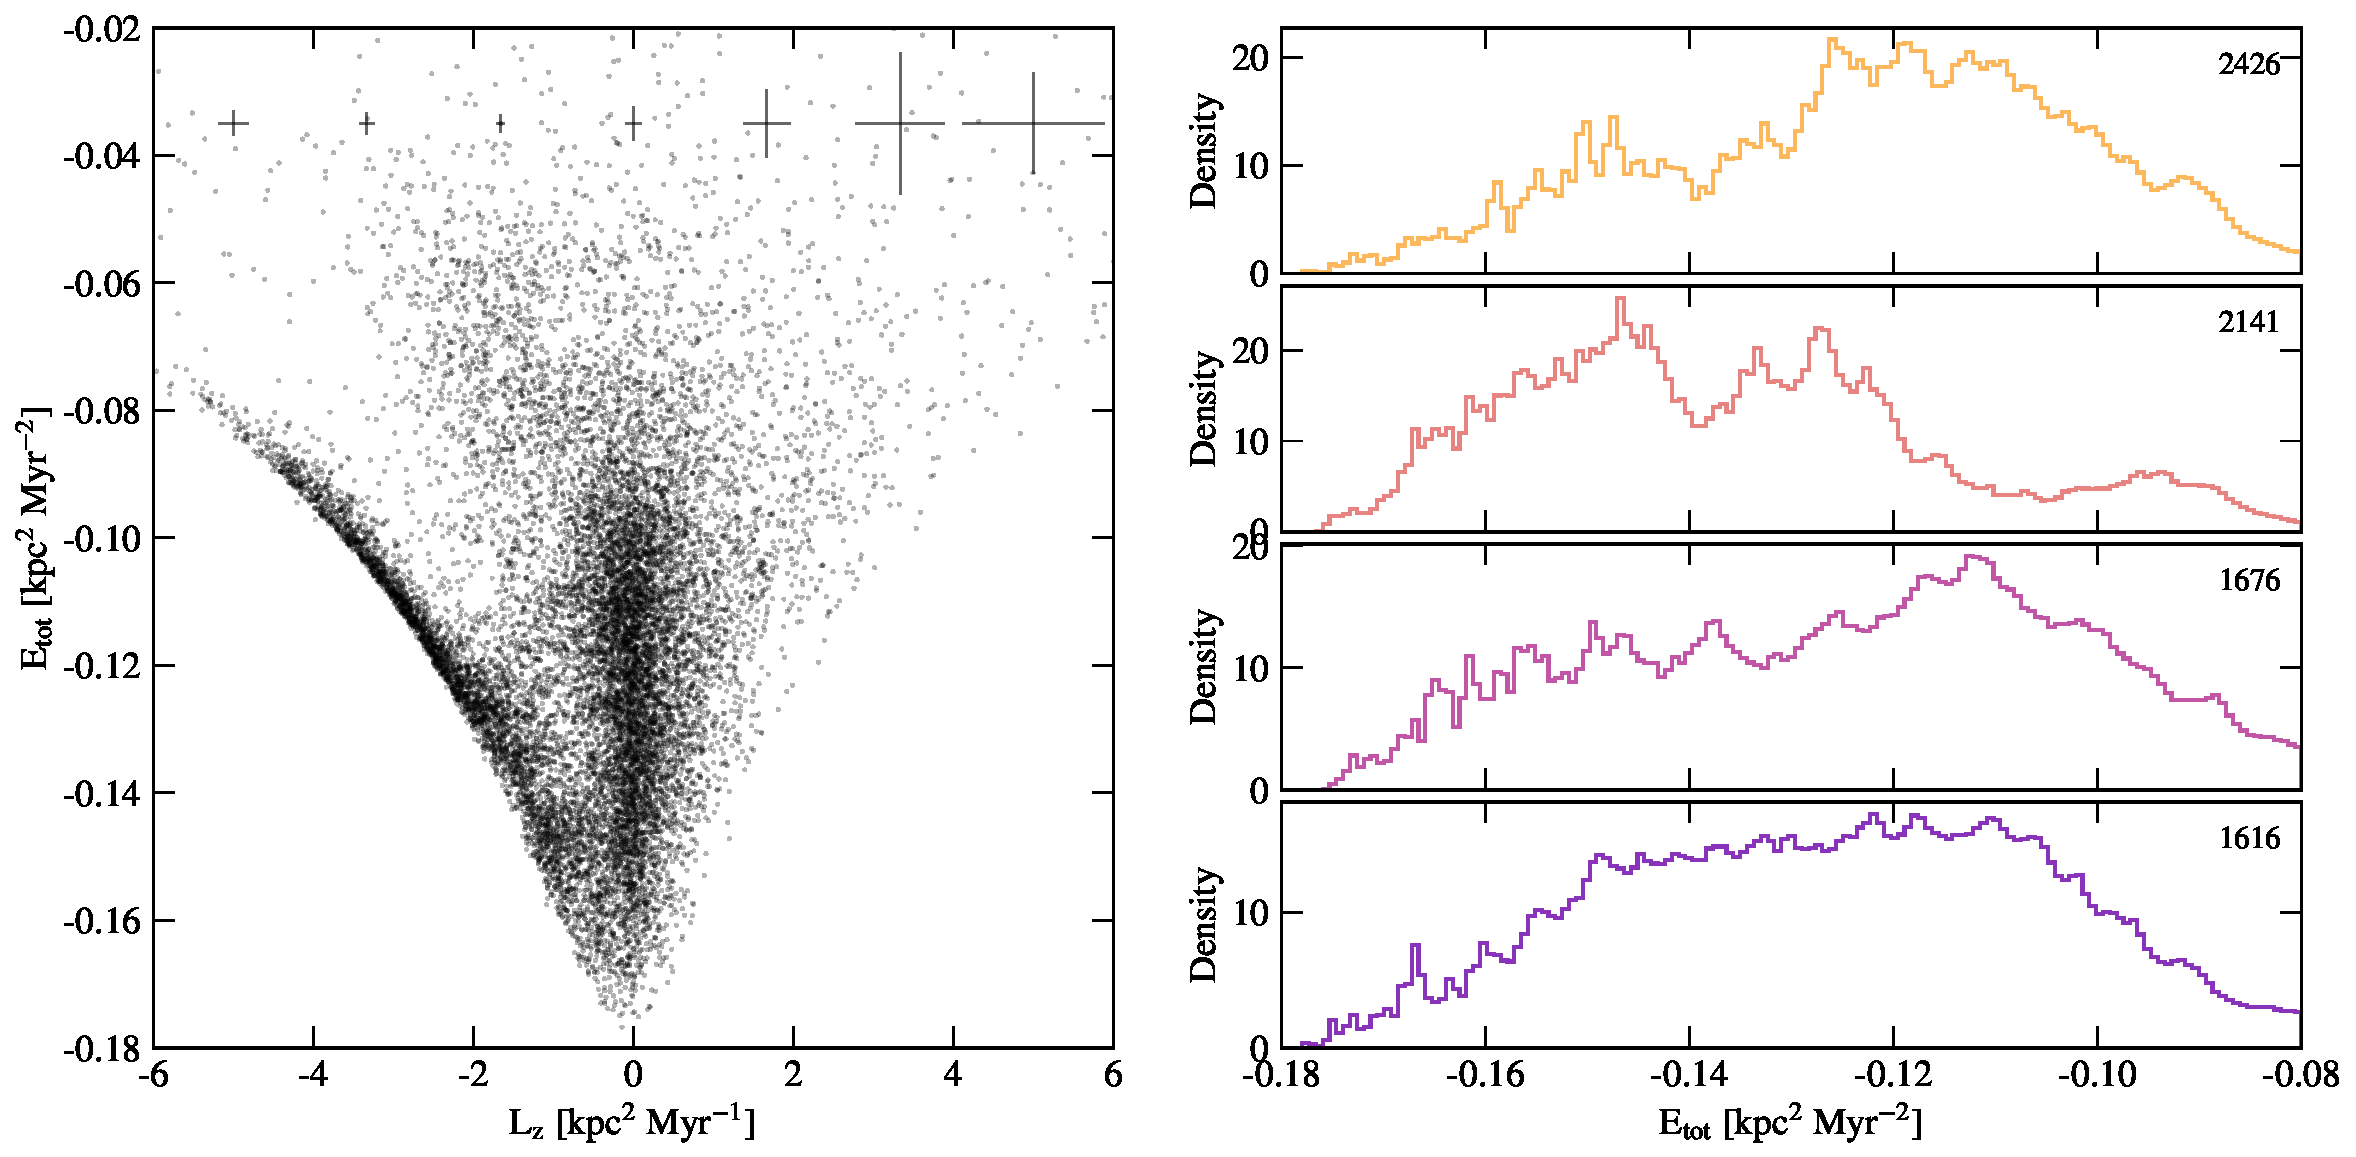
\includegraphics[width=0.95\textwidth]{fig1.pdf}
% \vspace{-4mm}
\caption{
\textbf{Orbital phase-space of Milky Way stars.}
{\bf Left panel:} Total orbital energies as a function of the $z$ component of orbital angular momentum (perpendicular to the Milky Way disk) of stars in the H3 survey.
Typical measurement uncertainties are shown as errorbars on top as a function of angular momentum.
- ripples
{\bf Right panels:} A resampled distribution of orbital energies, with each panel corresponding to a region of phase-space marked in the left panel.
The number of stars in each panel is indicated in the top right.
- best-fit model
}
% \vspace{-4mm}
\end{center}
\end{figure*}

- fig 1 shows E-Lz (2 panels: one points, another kde, annotated?)
- large scale clustering disk stars: left, GSE merger: center, retrograde shards: right, Sgr: top left + citations
- due to unprecedented precision (errorbars around the plot), we also detect small-scale clustering in the disk and the radial debris

- energy histograms (panel in fig 1)
- bootstraps
- fit mixture of gaussians
- auxiliary materials: non-bootstrapped version, function of snr; number of components

- why exciting: ringing -- disequilibrium easily mapped to dynamical history

- alternative: distinct accretion events
- smaller accretion events present, not obvious as overdensities\cite{naidu:2020}
- test through chemistry (fig 2)
- largely the same

- sim figure

- details of the simulation

- discrepancies

- comparison to other perturbations

- what we'll learn from this
-- subhalo survival related to expected dm annihilation rates)
-- vdbosch: Accurately predicting the demographics of dark matter (DM) substructure is of paramount importance for many fields of astrophysics, including gravitational lensing, galaxy evolution, halo occupation modelling, and constraining the nature of DM.
-- so far, dm tidal disruption only theoretical, plagued by resolution issues
-- here empirical!

%%%%%%%%%%%%%%%%%%%%%%%%%%%%%%%%%%%%%%%%%%%%%%%%%%%%

% \bibliographystyle{naturemag}
\bibliography{references}

\begin{addendum}
  
\item [Acknowledgements] 
% We thank both referees for their constructive
%   feedback.  C.C. is partially supported by the Packard
%   Foundation.  R.P.N. gratefully acknowledges an Ashford Fellowship
%   and Peirce Fellowship granted by Harvard University.  G.B.  and
%   N.G.-C. are supported by HST grant AR 15004, NASA ATP grant
%   17-ATP17-0006, NSF CAREER AST-1941096.  A.B. acknowledges support
%   from NASA through HST grant HST-GO-15930.  All the simulations were
%   run on El-Gato super computer which was supported by the National
%   Science Foundation under Grant No. 1228509.  We have made use of
%   data from the European Space Agency mission Gaia
%   (http://www.cosmos.esa.int/gaia), processed by the Gaia Data
%   Processing and Analysis Consortium (DPAC; see
%   http://www.cosmos.esa.int/web/gaia/dpac/consortium). Funding for
%   DPAC has been provided by national institutions, in particular the
%   institutions participating in the Gaia Multilateral Agreement.  This
%   publication makes use of data products from the {\it Wide-field
%     Infrared Survey Explorer}, which is a joint project of the
%   University of California, Los Angeles, and the Jet Propulsion
%   Laboratory/California Institute of Technology, and NEOWISE, which is
%   a project of the Jet Propulsion Laboratory/ California Institute of
%   Technology.  {\it WISE} and NEOWISE are funded by the National
%   Aeronautics and Space Administration.

\item[Author Contributions]
% C.C. and R.P.N. jointly conceived of the
%   project.  C.C. led the analysis of the data.  N.G-C. and
%   G.B. provided the simulation data and aided in its interpretation.
%   All authors contributed to aspects of the analysis and to the
%   writing of the manuscript.

\item[Author  Information]  
% Reprints and permissions
%     information is available at npg.nature.com/reprintsandpermissions.
%     Correspondence and requests for materials should be addressed to
%     C.C.\ (cconroy@cfa.harvard.edu).

\item[Data Availability] 
% The K giant catalog used in this paper is
%     available at \texttt{https://doi.org/10.7910/DVN/2D1H8J}.
    
\item[Code Availability] 
% We have opted not to make the code used in
%     this manuscript available because the data reduction and analysis
%     is straightforward and can be easily reproduced following the
%     methods described herein.
    
\end{addendum}


%%%%%%%%%%%%%%%%%%%%%%%%%%%%%%%%%%%%%%%%%%%%%%%%%%%%%%%%%%
%%%%%%%%%%%%%%%%%%%%%%%%%%%%%%%%%%%%%%%%%%%%%%%%%%%%%%%%%%

\newpage

\setcounter{page}{1}
\setcounter{figure}{0}
\setcounter{table}{0}
\captionsetup[figure]{labelformat=empty}
\renewcommand{\thefigure}{Extended Data \arabic{figure}}
\renewcommand{\thetable}{Extended Data \arabic{table}}

\begin{center}
{\bf \Large \uppercase{Methods}}
\end{center}

\noindent
{\bf Identification of giants / selection effects}

{\bf In-situ, bursty star formation?}

{\bf Bar?}

{\bf Dependence on the overall potential}


\end{document}



